\documentclass[a4paper,11pt]{article}
\usepackage{tabularx}
\usepackage{graphicx}
\usepackage{wrapfig}
\usepackage{subfigure}
\usepackage{enumerate}
\usepackage{natbib}
\usepackage[center,small]{caption}
\usepackage[top=2cm, bottom=2cm, left=2.5cm, right=2.5cm]{geometry} 

\title{\huge \textbf{Tutorial on using the \textit{spartan} package to analyse agent-based simulation results}\\
\Large For use with \textit{spartan} package version 1.2 onwards
\author{\Large Technique 1: Analysing Aleatory Uncertainty using SpartanV Interface}
\date{}
}
\begin{document}

\maketitle


\section{Introduction}
\noindent \textit{spartan}, or (\textbf{S}imulation \textbf{P}arameter \textbf{A}nalysis \textbf{R} \textbf{T}oolkit \textbf{A}pplicatio\textbf{N}) is an R package which aids the understanding of the effect aleatory and epistemic uncertainty have on the output from a simulation.  This set of tutorials makes use of available example simulation output to demonstrate how a variety of methods can be applied to further understand the results that have been generated.  Following through each example should make it easier to apply the tookit to results generated by any agent-based computer simulation.  This tutorial focuses on understanding the effect inherent stochasticity may have on simulation results, and uses a java based interface to spartan (SpartanV) to perform this analysis.

\section{The \textit{spartan} Package}
\noindent Computer simulations are becoming a popular technique to use in attempts to further our understanding of complex systems. This package provides code for four techniques described in available literature which aid the analysis of simulation results, at both single and multiple timepoints in the simulation run. The first technique addresses aleatory uncertainty in the system caused through inherent stochasticity, and determines the number of replicate runs necessary to generate a representative result. The second examines how robust a simulation is to parameter perturbation, through the use of a one-at-a-time parameter analysis technique. Thirdly, a latin hypercube based sensitivity analysis technique is included which can elucidate non-linear effects between parameters and indicate implications of epistemic uncertainty with reference to the system being modelled. Finally, a further sensitivity analysis technique, the extended Fourier Amplitude Sampling Test (eFAST) has been included to partition the variance in simulation results between input parameters, to determine the parameters which have a significant effect on simulation behaviour.

\section{The Case Study}
\noindent The example simulation results have been taken from an ongoing project which seeks to understand the formation of lymphoid tissue in the small intestine. This simulation outputs cell behaviour measures at various points in the simulation and measures describing the development of the tissue, which occurs through interactions between the cells. Techniques 2-4 of this package allow us to explore how input parameter value affects the behaviour of these cells. We need Technique 1 to tell us how many simulation runs we need for each condition explored to ensure we have a robust representative result.

\section{Scope}
\noindent Do note that the idea of this tutorial is to demonstrate the application of the toolkit, and is not intended to act as a full introduction to using Sensitivity Analysis techniques in the analysis of simulation results. Where useful, links to further reading have been included.

\section{Prerequisites}
\begin{itemize}
\item The R statistical environment, version 2.13.1 or later.
\item The spartan R package, downloaded from the Comprehensive R Archive Network (CRAN) or from the project website.
\item The lhs and gplots R packages, available for download from CRAN.
\item The example simulation results, available from the project website.
\item From version 1.2 of \textit{spartan}, simulation results can be in either CSV or XML format. For earlier versions, results must be pre-processed to be in CSV format.
\item The SpartanV Java Interface for the spartan package. Please make sure you follow the installation instructions fully prior to running this tutorial.
\end{itemize}

\section{Running Technique 1: Aleatory Analysis (AA)}
\noindent Aleatory uncertainty can be caused by inherent stochasticity within a simulation. This is especially the case for agent-based simulations, where different results will be gained although the same parameter input values used. Thus a number of replicate simulation runs need to be performed to achieve a representative result. This technique gives an indication of the number of simulation runs necessary to reduce this uncertainty. This follows the method described by Read et al (2012).  Note at this stage we are not concerned with parameter sensitivity, more producing a representative result.  Thus this analysis uses the simulation parameters set through some process of calibration.\\
\\
To use this, you should have chosen the number of replicate runs to analyse. For example, in this tutorial we examine 1, 5, 50, 100 and 300 replicates of a simulation under the same parameter conditions.  For each sample, twenty sets of results are created, with each set containing the number of simulation results for that sample size.  So, we have 20 sets where the simulation was run once, 20 sets where each set contains the results of 5 runs, right through to 20 sets where each contains the results of 300 runs. The technique then looks at each sample size used, and (a) generates the median distribution for all output measures for each of the twenty subsets (b) goes through each of the subsets, comparing the median distribution of each measure with the respective median distribution in the first subset using the Vargha-Delaney A-Test (2000) which gives an indication of how different the results are, (c) for each sample size, creates a graph showing how different the results of each subset are (i.e. the A-Test result).\\
\\
This section of the tutorial performs this analysis for the lymphoid tissue formation simulation, which has been developed using an agent-based approach. In this case, we are going to examine two cell behaviour measures, Velocity and Displacement, that are captured for a simulation period representing one hour. In the simulation results folders, the file we are going to look at is trackedCells\_Close.csv.

\begin{figure}
\centering
    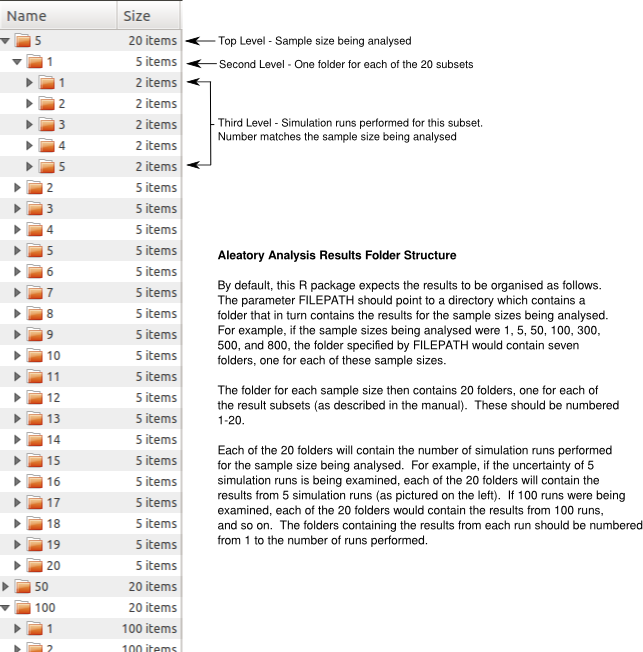
\includegraphics[width=\textwidth]{AA_Folder_Struc.png}\\ \noindent
    \caption{Simulation results folder structure that should exist for use with this tool}
    \label{AA_Folders}
    \newpage 
\end{figure}

\begin{enumerate}
\item Download the AA example result set from the project website and extract the results.
\item The first thing to note is the folder structure.  To use this method, the simulation results do need to be in a specific format (Figure \ref{AA_Folders} – AA folder structure).  The structure has three levels:
\begin{enumerate}[(i)]
\item Folders for each sample size being analysed
\item Twenty folders, one for each of the subsets within that sample size
\item A folder for each of the simulation results in that subset.  So, if you are analysing five simulation results, there will be 5 folders, numbered 1-5. 
\end{enumerate}
\item With this data available, open the SpartanV Java Interface for Spartan. From the analysis method choices, select the first option "Aleatory Uncertainty Analysis". Now we are going to declare the R variables required to run this analysis. The first screen requests information on where the simulation results are stored, how many runs have been performed, and what the simulation output responses are. Use the directory browser to select the directory where you extracted the tutorial data. For the remaining inputs, Figure \ref{AA_Screen1} shows the responses that should be entered for this scenario. Complete this screen and press next.

\begin{figure}
\centering
    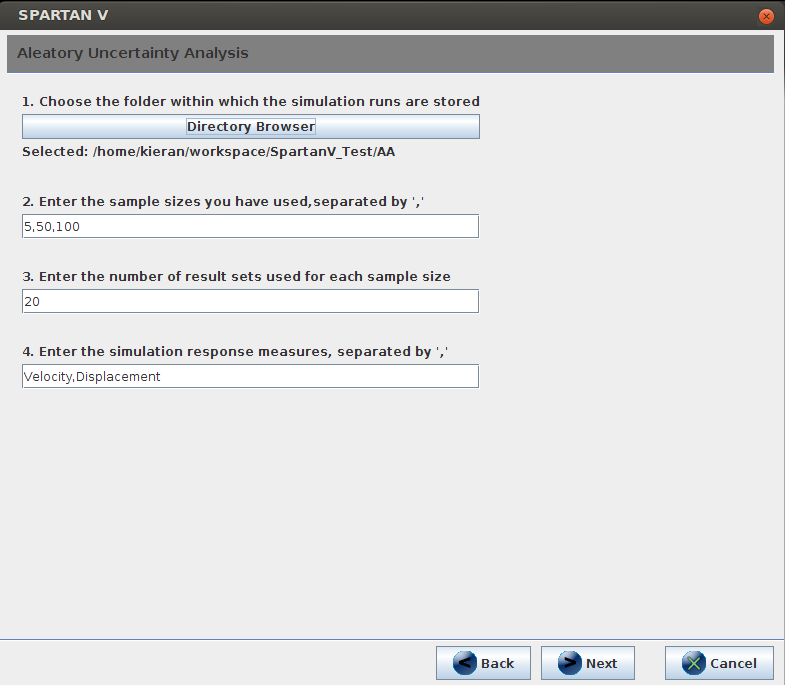
\includegraphics[width=0.8\textwidth]{SpartanV_AA1.png}\\ \noindent
    \caption{Responses for R variables on the first input screen}
    \label{AA_Screen1}
    \newpage 
\end{figure}

\item The second screen requests information about the simulator, in terms of output type (spartan can process XML or CSV), result file names, and particular columns where the output responses can be found (if csv). For CSV output, it is good to specify result start and end columns to save R errors on duplicate first column entries, and to save reading in whole CSV files. Finally, the screen requests information on simulation timepoints that are being examined. This is covered later in the tutorial. In this scenario, we assume we are only examining one timepoint, and this the last two input boxes are set to NULL. Complete the input boxes with the data shown in Figure \ref{AA_Screen2} and click Next.

\begin{figure}
\centering
    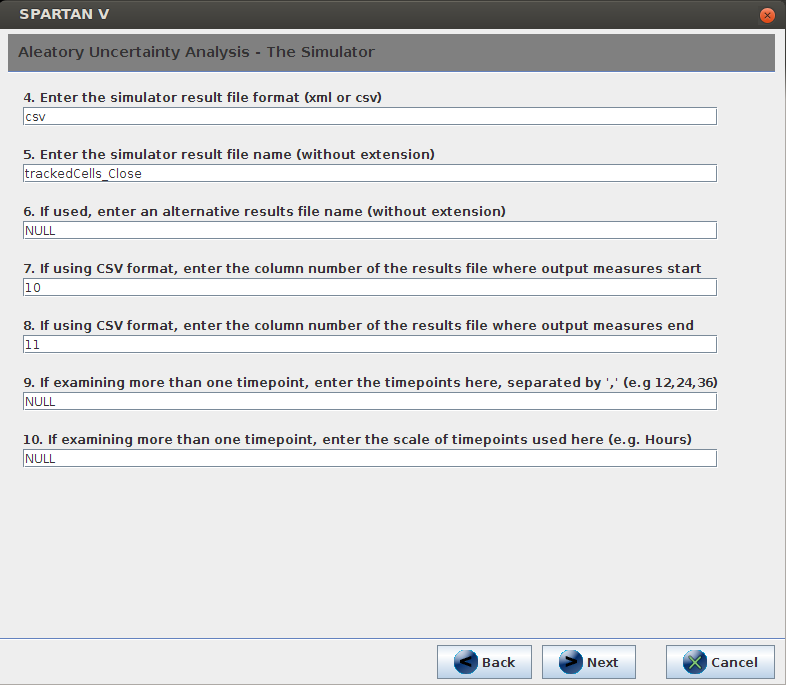
\includegraphics[width=0.8\textwidth]{SpartanV_AA2.png}\\ \noindent
    \caption{Responses for R variables on the second input screen}
    \label{AA_Screen2}
    \newpage 
\end{figure}

\item Screen 3 asks you to specify the names assigned to the files output by spartan. The first asks for the format you wish the median output responses for each simulation run size subset to be in. This can be CSV or XML. The other entry boxes specify names of the A-Test result files for each sample size and names of the plots that are produced. Complete this screen such that it contains the responses shown in Figure \ref{AA_Screen3} and press Next.

\begin{figure}
\centering
    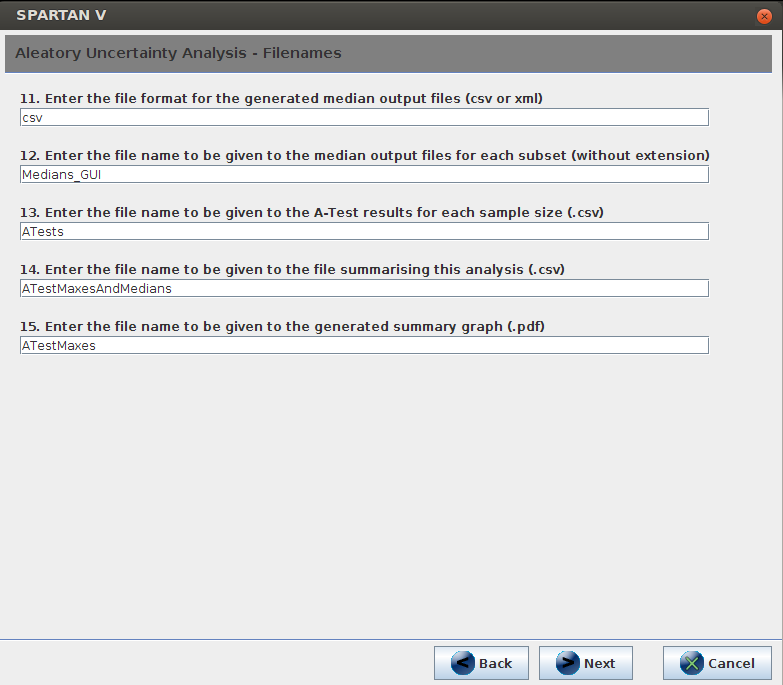
\includegraphics[width=0.8\textwidth]{SpartanV_AA3.png}\\ \noindent
    \caption{Responses for R variables on the third input screen}
    \label{AA_Screen3}
    \newpage 
\end{figure}

\item Screen 4 concerns the statistical significance limits applied by the Vargha-Delaney A-Test. These are set at the default values but can be changed here if it proves necessary. In this case, leave these at the default values (in Figure \ref{AA_Screen4}) and press Next.

\begin{figure}
\centering
    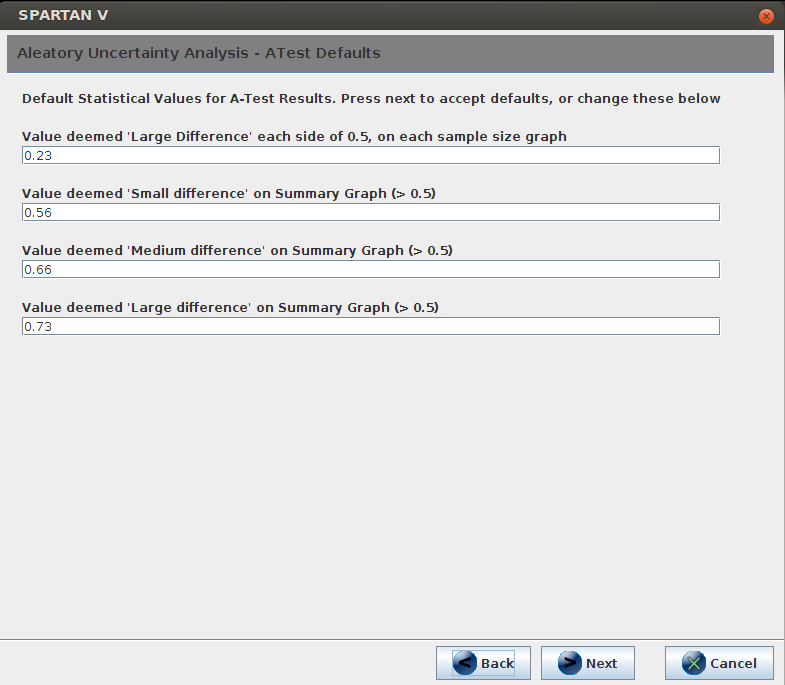
\includegraphics[width=0.8\textwidth]{SpartanV_AA4.png}\\ \noindent
    \caption{Responses for R variables on the fourth input screen}
    \label{AA_Screen4}
    \newpage 
\end{figure}

\item The final screen asks what methods you wish to run in this analysis. Although you would normally run them all, you may want to run some of these separately, or perform them at different times. In this case, we are going to run all three. These are:

\begin{verbatim}
aa_analyse_all_sample_sizes(FILEPATH, SAMPLESIZES, NUMSUBSETSPERSAMPLESIZE,
RESULTFILEFORMAT, RESULTFILENAME, ALTFILENAME, OUTPUTFILECOLSTART,
OUTPUTFILECOLEND, MEASURES, MEDIANSFILEFORMAT,MEDIANSFILENAME,
ATESTRESULTFILENAME, LARGEDIFFINDICATOR)
\end{verbatim}

This independently examines each sample size to be examined, and determines how 'different' the results of each of the 20 subsets are.  As a first step, the algorithm needs to go through each subset and create a set of medians which can then be compared with another of the 20 subsets. Therefore, the algorithm takes each of the 20 sets in turn, producing a file containing the median of each output measure for each simulation run in that set. This may be easier to understand with the use of an example. Lets say we are analysing the uncertainty in 5 simulation runs. So our sample size is 5.  For this sample size, we will have 20 sets of results, each containing 5 runs. The algorithm takes each of these 20 in turn, producing a file containing the median output for all measures for each of the 5 runs. (so, in our example, we have two output measures, Velocity and Displacement - a file would be created within each of the 20 sets containing the median Velocity and Displacement measures for each of the 5 runs).  Once this process has been completed, the median results for subsets 2-20 are compared with those in subset 1 using the Vargha-Delaney A-Test, with these results stored in an output file. This file is either in CSV or XML format, dependent on the file format set in the MEDIANSFILEFORMAT variable. The A-Test results are then graphed, showing how different each of the 20 subsets are. Thus, when this example is run, you will generate five graphs, one for each sample size.  

\begin{verbatim}
aa_sampleSizeSummary(FILEPATH,SAMPLESIZES,MEASURES,ATESTRESULTFILENAME,
SUMMARYFILENAME)
\end{verbatim}

This will produce, in the top level of the folder structure, a csv file named as specified by the Summary File name input box  (EgSet\_ATestMaxAndMedians.csv in this case). When you open this CSV file when we have performed the next step, you will see it contains both the maximum and median A-Test scores over the 20 subsets for each output measure, and for each sample size. Alongside these values you will also find a 'Normalised' value.  With the A-Test, a result of 0.5 implies there is no significant difference.  The directionality of results either side of this is not important, and therefore these can be normalised so that all A-Test maximum and median values are above 0.5.

\begin{verbatim}
aa_graphSampleSizeSummary(FILEPATH,MEASURES,MAXSAMPLESIZE,SMALL, MEDIUM, LARGE, 
SUMMARYFILENAME, GRAPHOUTPUTFILE, TIMEPOINTS,TIMEPOINTSCALE)
\end{verbatim}

This will produce a summary graph in the top level of the folder structure containing the maximum A-Test value observed over the 20 subsets for each sample size. All being well, you should see the score decrease as sample size increases.  \\

\item Press Next. On the final screen, press the "Run Aleatory Analysis" button. The console screen will show the progress of this analysis.
\\
For the set of parameters specified above, this will produce:
\begin{enumerate}[(i)]
\item Median results files within each of the 20 folders within each sample size - named as stated in the MEDIANSFILENAME variable (EgSet\_Median.csv in this case)
\item A graph within each sample size, showing 'how different' result sets 2-20 are in comparison with the results in subset 1.  These graphs should be named \textit{n}Samples.pdf. An example can be seen in Figure \ref{AA_5Samples}.
\item A summary graph showing the maximum A-Test score seen for each sample size. An example can be seen in Figure \ref{AA_Results}
\end{enumerate}. 
\\

Your aim is to find a sample size which minimises the A-Test value for all measures.  In this example case, we did not deem 300 runs to be sufficiently close enough to the 'no difference' line for both Velocity and Displacement measures, and did the same analysis with 500 runs.  However, this value will be different for all simulations that are analysed this way.


\end{enumerate}
\newpage 
\begin{figure}[h!]
\centering
    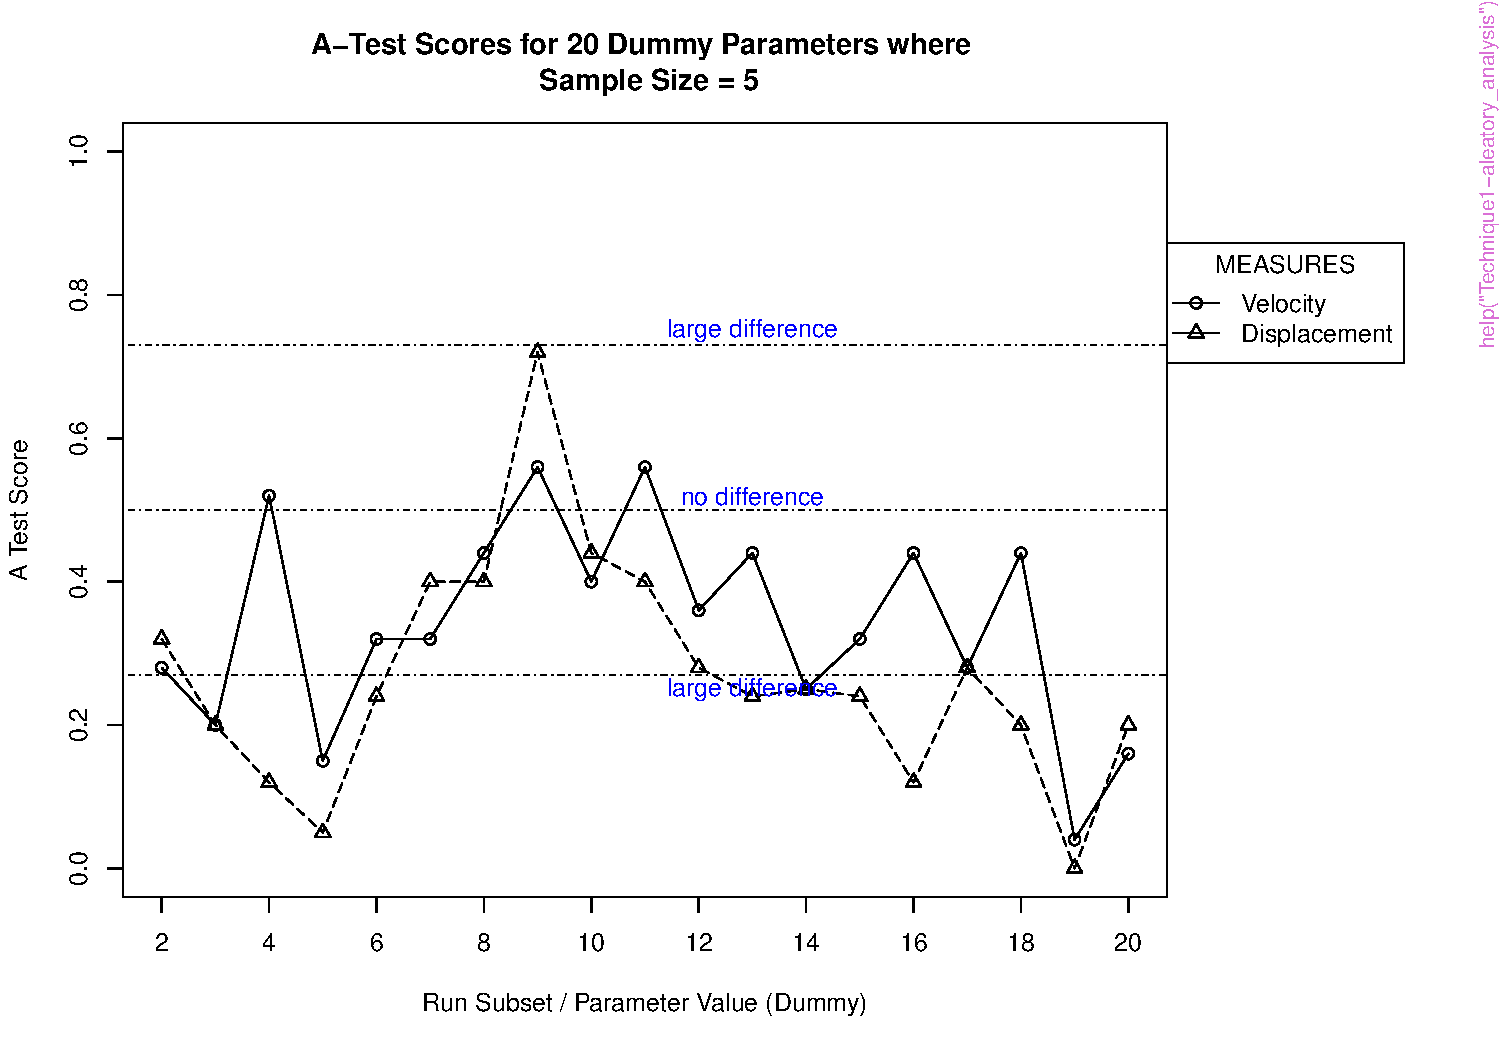
\includegraphics[width=0.9\textwidth]{AA_5Samples.pdf}\\ \noindent
    \caption{Graph showing the A-Test scores where sample sets 2-20 are compared with the first sample set}
    \label{AA_5Samples}
    \end{figure}

\begin{figure}[h!]
\centering
    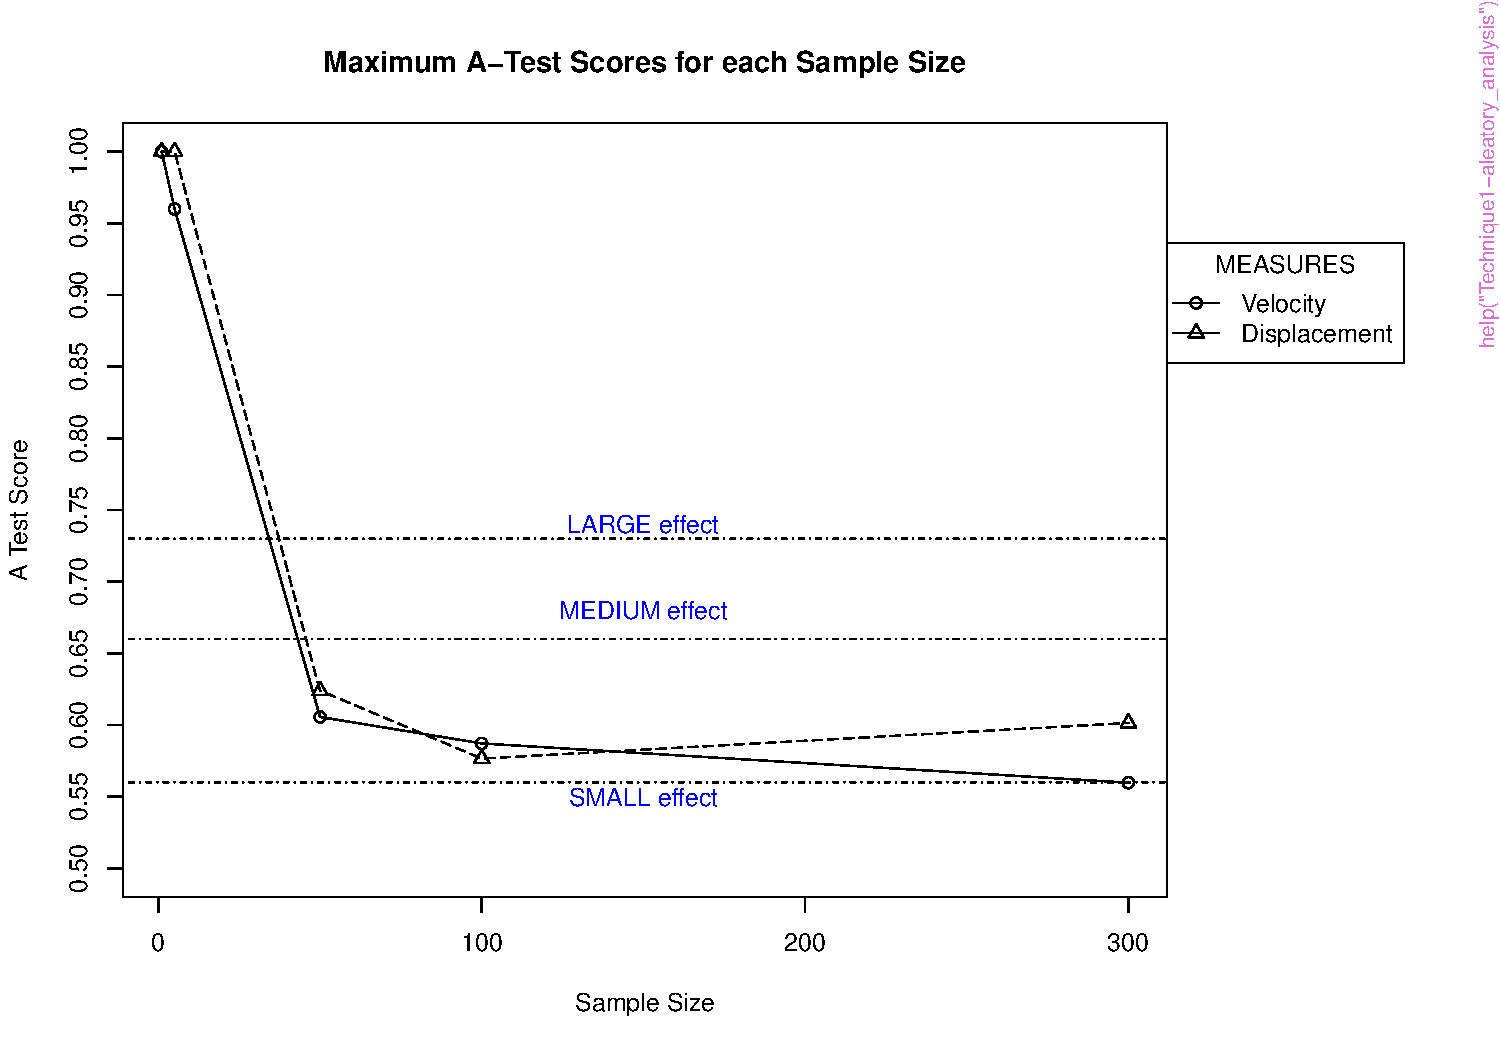
\includegraphics[width=0.9\textwidth]{AA_Results.pdf}\\ \noindent
    \caption{Graph summarising the maximum A-Test result observed over the 20 subsets, for all sample sizes}
    \label{AA_Results}
\end{figure}

\section{Running AA Technique for Multiple Timepoints}
\noindent The package also has the capability to perform the above analysis for simulation results taken at different timepoints. This may give an indication of when such variance becomes an influential.  Again, we will examine this with an example, yet there is not much to change from the example seen previously.
\\
In this case study, we have captured the cell behaviour measures at multiple timepoints in the simulation, specifically 12, 36, 48,and 60 hours.  Thus we have the output files trackedCells\_Close\_12.csv, trackedCells\_Close\_36.csv etc. To use this method over multiple timepoints, you should have (a) the same folder structure as in the previous example, and (b) an output file for each timepoint, with the timepoint appended to the filename after an underscore. It is worth writing a script to put your output in this format before looking at this method if that is not already the case
\\
Launch the SpartanV interface, and complete Steps 1-3 in the same way as that above. Now, on the second data input screen, enter 12,36,48,60 into box 9 (Timepoints) and type Hours into box 10 (timepoint scale), as seen in Figure \ref{AA_Screen5}. This tells the analysis that you want to examine simulation responses at four different time-points, with the latter used for graphing results in the final part of the method. Press Next and complete the other data entry screens in the same way. Run the analysis, and statistics will be produced for all four timepoints.

\begin{figure}
\centering
    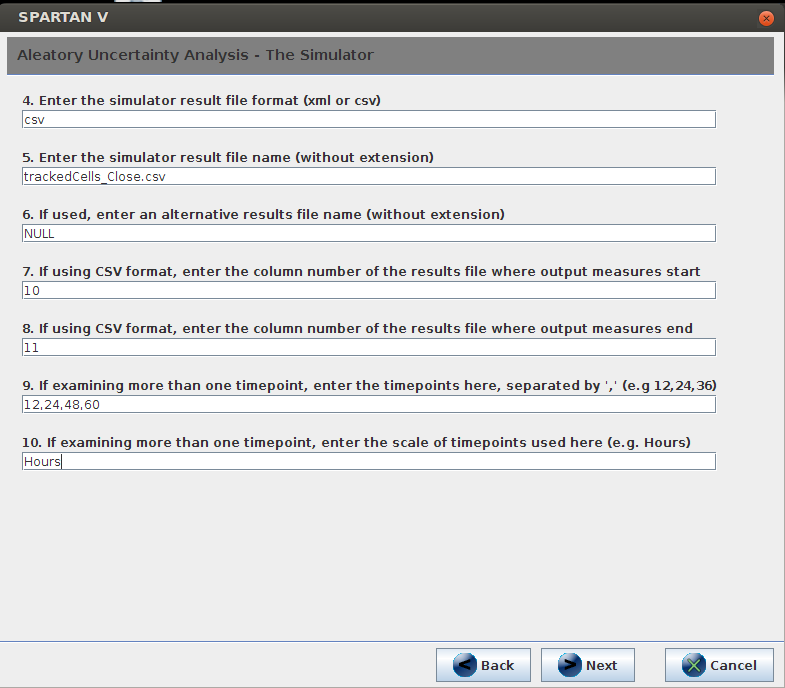
\includegraphics[width=0.8\textwidth]{SpartanV_AA5.png}\\ \noindent
    \caption{Analysing simulation responses at different timepoints}
    \label{AA_Screen5}
    \newpage 
\end{figure}

\section{Further Reading}
\noindent
The following two references may be useful in understanding this technique in more detail:
\begin{itemize}
\item Read, M., Andrews, P.S., Timmis, J. \& Kumar, V. (2012) Techniques for Grounding Agent-Based Simulations in the Real Domain : a case study in Experimental Autoimmune Encephalomyelitis. Mathematical and Computer Modelling of Dynamical Systems, 18(1):67-86.
\item Vargha, A. \& Delaney, H.D. (2000) A critique and improvement of the CL Common Language Effect Size Statistics of McGraw and Wong. Journal of Educational and Behavioural Statistics, 25, p.pp.101-132.
\item The spartan Manual, spartan-Manual.pdf, within the spartan package describes in more detail each method within the package
\end{itemize}


\end{document}